\section{Results}
To evaluate GBD as a viable physical optics propagation technique we must evaluate its performance v.s. Fresnel diffraction for a given observatory. The fiducial observatory used in this study is a Ritchey-Chretien (RC) objective based on the Hubble Space Telescope (HST). This model is developed both in Zemax OpticStudio and as a paraxial optical system to compare the propagation methods. The system prescription is given in table \ref{tab:fiducial_observatory_specs} and the effective ray transfer matrix is given in equation \ref{eq:hstrtm}. 

\begin{table}[H]
    \centering
    \begin{tabular}{c c c c c}
        \hline
        Surface & RoC [m] & Conic Constant & Distance [m] & Semi-Aperture [m]  \\
        \hline
        M1 & -11.0400 & -1.00230 & -4.90607 & 1.20000 \\
        M2 & -1.35800 & -1.49686 &  6.40620 & 0.14056 \\
        \hline
        \\
    \end{tabular}
    \caption{Optical system prescription for the RC telescope based on the HST used in this investigation. All distances are given in meters. }
    \label{tab:fiducial_observatory_specs}
\end{table}

\begin{equation}
    \mathbf{O_{RC}} =
    \begin{pmatrix}
    0 & 0 & 57.6 & 0 \\
    0 & 0 & 0 & 57.6 \\
    -0.0174 & 0 & 1 & 0 \\
    0 & -0.0174 & 0 & 1 \\
    \end{pmatrix}
    \label{eq:hstrtm}
\end{equation}

% \begin{table}[H]
%     \centering
%     \begin{tabular}{c c}
%     \hline
%         Parameter & Value  \\
%          \hline
%         Focal Length & 57.6000 \\
%         Entrance Pupil Diameter & 2.4 \\
%         \hline
%         \\
%     \end{tabular}
%     \caption{Caption}
%     \label{tab:my_label}
% \end{table}

The equivalent paraxial optical system (Fresnel, paraxial GBD) can't be easily modeled because the mirrors aren't well-represented by the quadratic phase surface characteristic of thin lenses in diffraction modeling software. Rather, the observatory will be modeled as though it was a single thin lens inside the entrance pupil of the telescope with focal length equal to the total focal length of the telescope. Aberrations are applied to the non-paraxial model by perturbing the position of the secondary mirror. The same aberrations are applied to the paraxial models by doing a Zernike polynomial decomposition on the wavefront phase in the exit pupil. These phase aberrations are applied in the pupil of the paraxial model and propagated to focus.

\subsection{The Fiducial Coronagraph}

The fiducial coronagraph for this study is a charge-2 vector vortex coronagraph (VVC). The complex amplitude of the focal plane mask is 

\begin{equation}
	U(x,y) = exp[i 2 arctan(\frac{y}{x})]
\end{equation}

and the transmission is unity everywhere except for the center pixel, where it is 0. This is because there is a singularity in the phase ramp at this location, so it must be masked out. We chose the VVC because of its ability to effectively reject on-axis starlight at a given wavelength. Should GBD introduce undesirable artifacts into the PSF, it should be visible in the coronagraphic focal plane. The VVC used in this simulation necessitated very high sampling (16k x 16k array) in order to resolve the singularity.

\label{sect:results}  % \label{} allows reference to this 
\subsection{Paraxial Model}

The Fresnel-equivalent models of the observatory PSFs and the coronagraphic PSFs for our HST model with a circular aperture are shown below in figures \ref{fig:paraxial_psfs} and \ref{fig:paraxial_coronagraph}, respectively. The observatory PSF comparison in figure \ref{fig:paraxial_psfs} has the analytical airy function for an equivalent telescope aperture subtracted to reveal the computational residuals from using this diffraction method.

\begin{figure}[H]
    \centering
    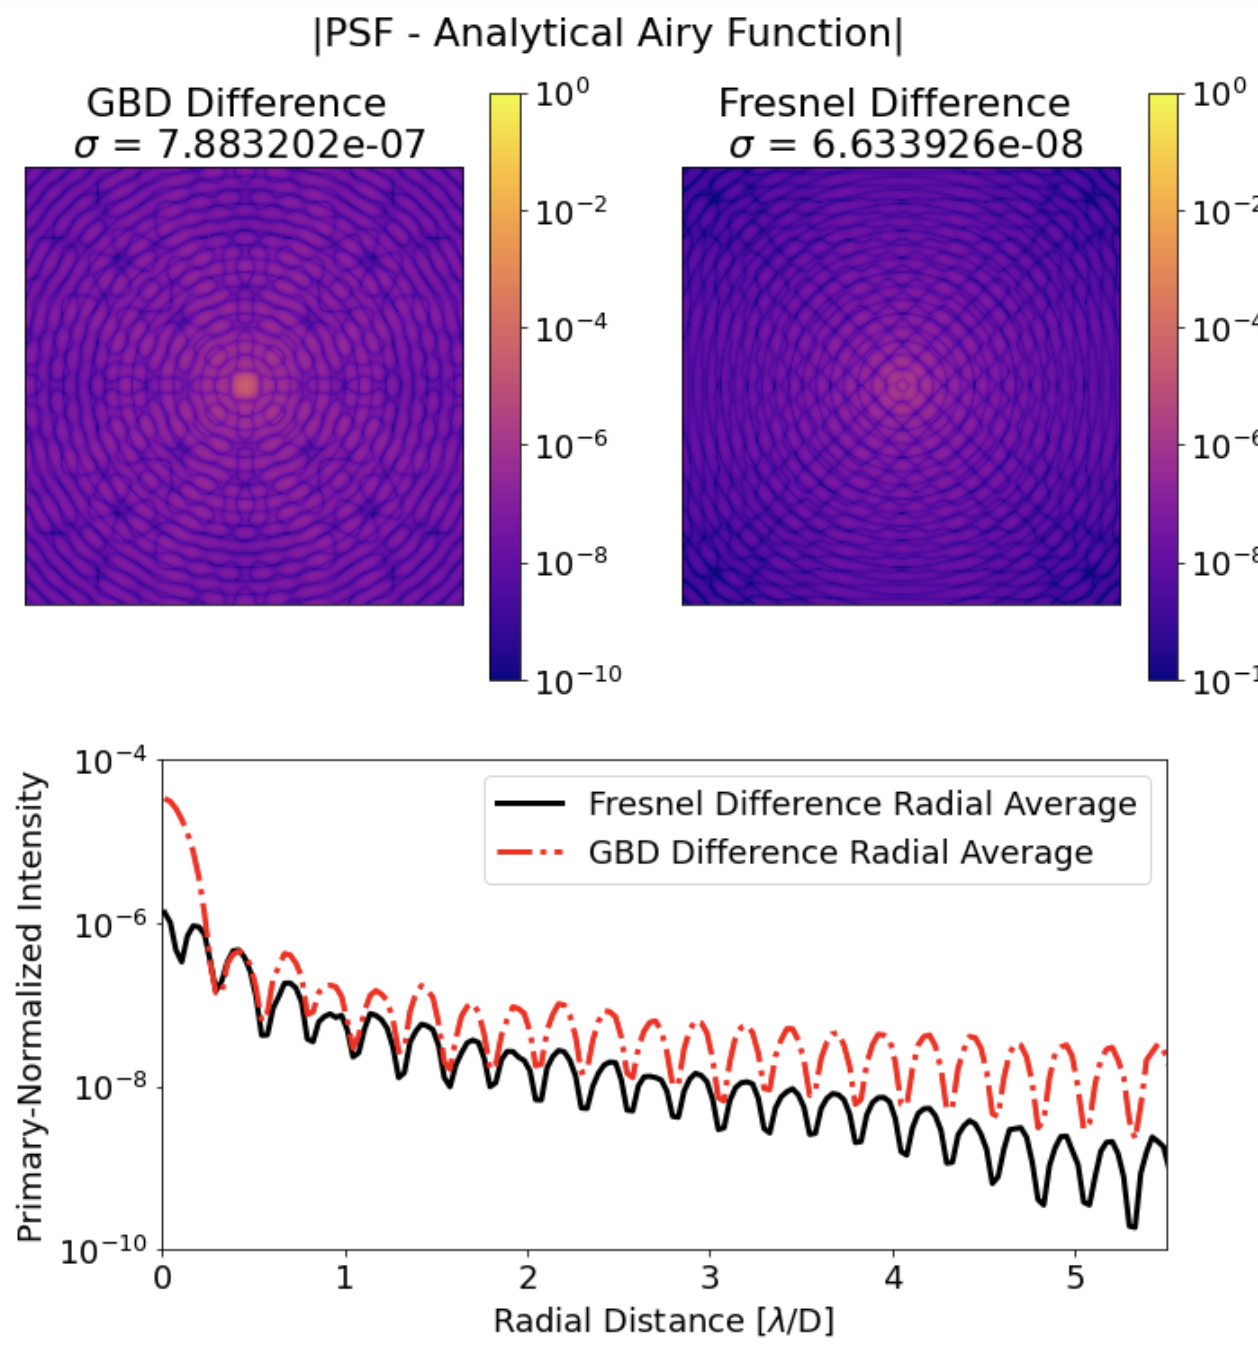
\includegraphics[width=0.7\textwidth]{paraxial_psf_record_9200wo.png}
    \caption{Comparison of the PSF generated by paraxial GBD (left) and Fresnel (middle) for the same optical system with the analytical result subtracted. The azimuthally averaged radial profile is plotted to clarify the discrepancy in the PSF (bottom). }
    \label{fig:paraxial_psfs}
\end{figure}

Neither reproduce the airy function exactly, which is an expectation of any finite simulation. The discrepancy in the GBD PSF comes from the characteristic ripple from the beamlet distribution, and the inability to fully reconstruct a sharp-edge aperture. The discrepancy in the Fresnel PSF comes from the discretization of the circular pupil. Both simulations can be improved by higher sampling, but this comes as substantially greater computational cost. To understand the influence of these residual errors they must be propagated through the fiducial coronagraph model. We also inject a faint and incoherent off-axis source for this simulation to illustrate a case of imaging a planetary companion. 

%\begin{figure}[H]
%    \centering
%    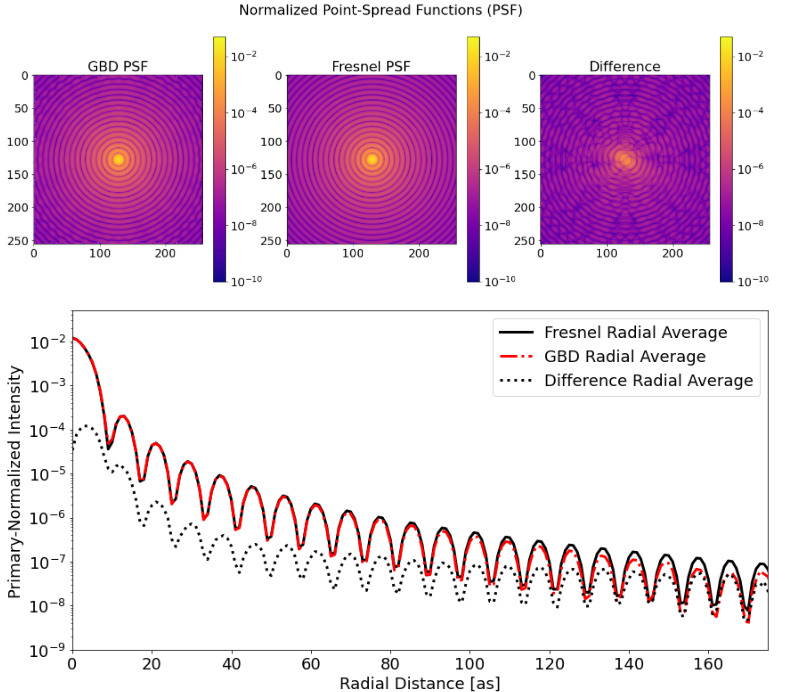
\includegraphics[width=\textwidth]{paraxial_waberration.png}
%    \caption{Comparison of the PSF \emph{with} aberration generated by paraxial GBD (left) and Fresnel (middle) for the same optical system and the difference of the PSFs (right). The azimuthally averaged radial profile is plotted to clarify the discrepancy in the PSF (bottom).}
%    \label{fig:paraxial_psfs_wabb}
%\end{figure}

% Might need to oversample a bit more so that the cross pattern isn't there
\begin{figure}[H]
    \centering
    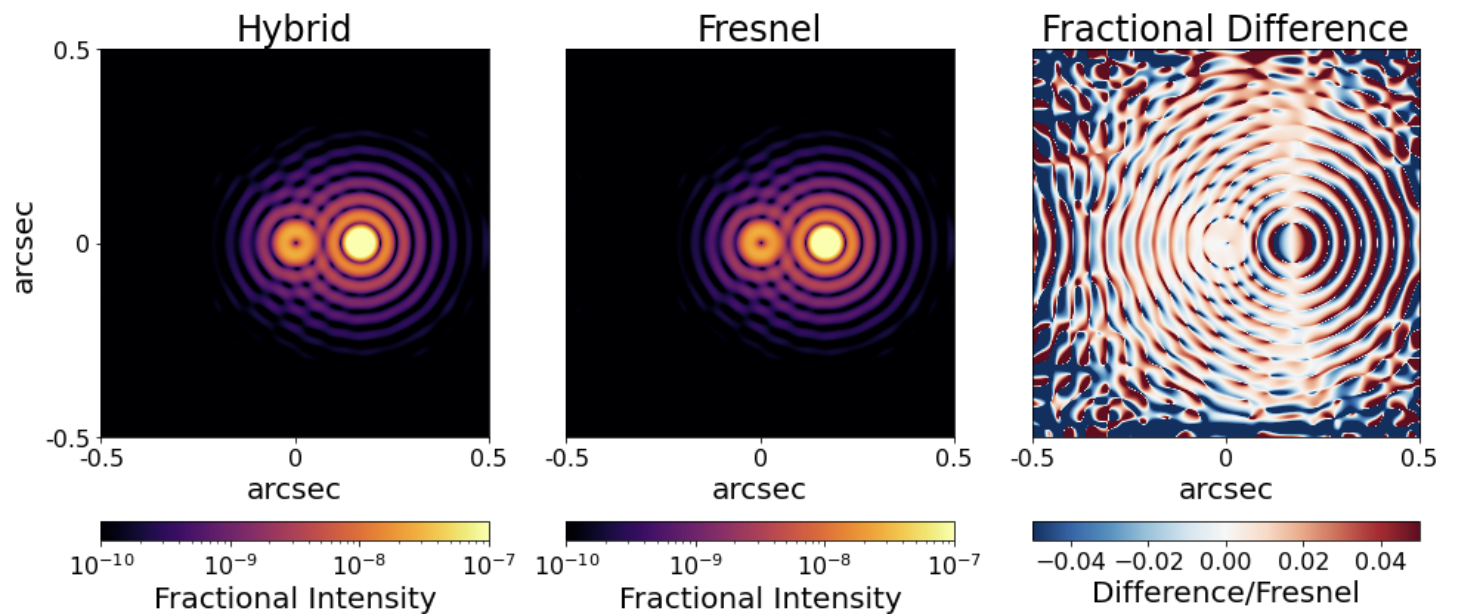
\includegraphics[width=\textwidth]{paraxial_vvc_compare.png}
    \caption{Comparison of the Coronagraphic PSF without aberration generated by paraxial GBD (left) and Fresnel (middle) and the fractional difference of the PSFs (right). The RMS difference of the PSFs is on the order of $3 \times 10^{-11}$.}
    \label{fig:paraxial_coronagraph}
\end{figure}

The coronagraphic images show an encouraging congruence. By inspection the images shown in Figure \ref{fig:paraxial_coronagraph} are nearly identical. The fractional difference shows that where there is actually power in the image the difference is negligible, indicating the suitability of the proposed hybrid propagation scheme for creating fresnel-equivalent models of observatories outfitted with coronagraphs.

%\begin{figure}[H]
%    \centering
%    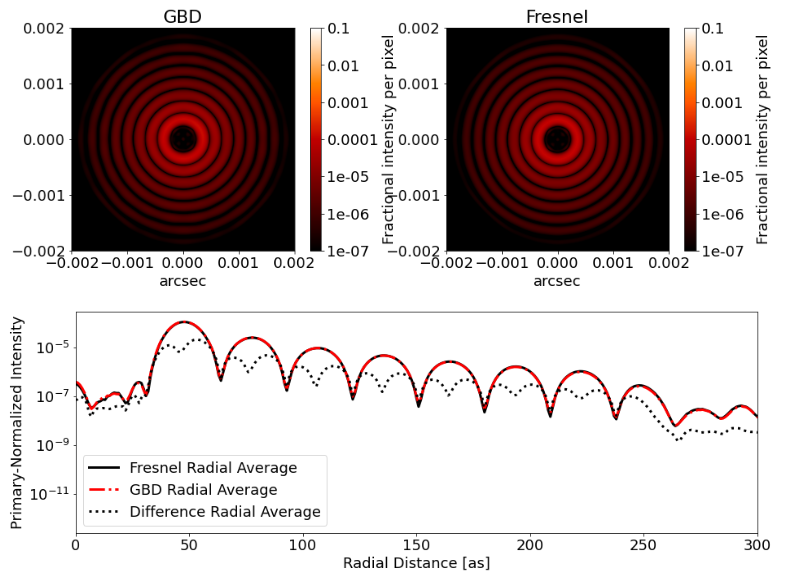
\includegraphics[width=\textwidth]{coron_paraxial_withabberation.png}
%    \caption{Comparison of the Coronagraphic PSF with aberration generated by paraxial GBD (left) and Fresnel (middle) and the difference of the PSFs (right). The azimuthally averaged radial profile is plotted to clarify the discrepancy in the PSF (bottom).}
%    \label{fig:paraxial_coronagraph_wabb}
%\end{figure}

\subsection{Real Model}

While the paraxial results are an encouraging first demonstration of GBD's ability to accurately simulate an observatory PSF, the real power of the technique lies in its ability to connect a Fresnel model of a coronagraph to a ray trace model of an observatory. Shown below are the PSF simulations using the differential ray tracing methods detailed in Section 2. 

\begin{figure}[H]
    \centering
    % \includegraphics{}
    \caption{Comparison of the PSF generated by non-paraxial GBD (left) and Fresnel (middle) for the same optical system and the difference of the PSFs (right). The azimuthally averaged radial profile is plotted to clarify the discrepancy in the PSF (bottom).}
    \label{fig:nonparaxial_psf}
\end{figure}

\begin{figure}[H]
    \centering
    % \includegraphics{}
    \caption{Comparison of the Coronagraphic PSF generated by non-paraxial GBD (left) and Fresnel (middle) for the same optical system and the difference of the PSFs (right). The azimuthally averaged radial profile is plotted to clarify the discrepancy in the PSF (bottom).}
    \label{fig:nonparaxial_coronagraph}
\end{figure}